
\chapter{Standard Model of Electroweak Interation}
The standard model (SM) of particle physics represents our best understanding of elementary particles and their interactions. It is one of the most successful theories, because its predictions are confirmed with exceptional precision in many experiments. The SM is a gauge quantum field theory with gauge symmetry $SU(3)_C \otimes SU(2)_L \otimes U(1)_Y$\cite{Glashow1961,Weinberg,Salam,GIM,GG,Pol,Pol1,GrossWil,GrossWil1, SWQCD, SWQCD1,SW,thooft1,thooft2,tHooftVeltman,tHV}. $SU(3)_C$ is the gauge symmetry of quantum chromdynamics (QCD), the theory describing strong interactions, and $SU(2)_L \otimes U(1)_Y$ is the gauge symmetry of electroweak interactions. The SM is contructed by invariance under Poincare group (translations, rotations and Lorentz boosts) and renormalizablity. The constituents of matter are spin-$1/2$ particles (fermions), 6 leptons and 6 quarks that pair up to transform under $SU(2)_L$. The interactions of SM are mediated by spin-$1$ particles-gauge bosons. The elementary particles of the SM are listed in Figure 1.1.
\begin{figure}
	\begin{center}
		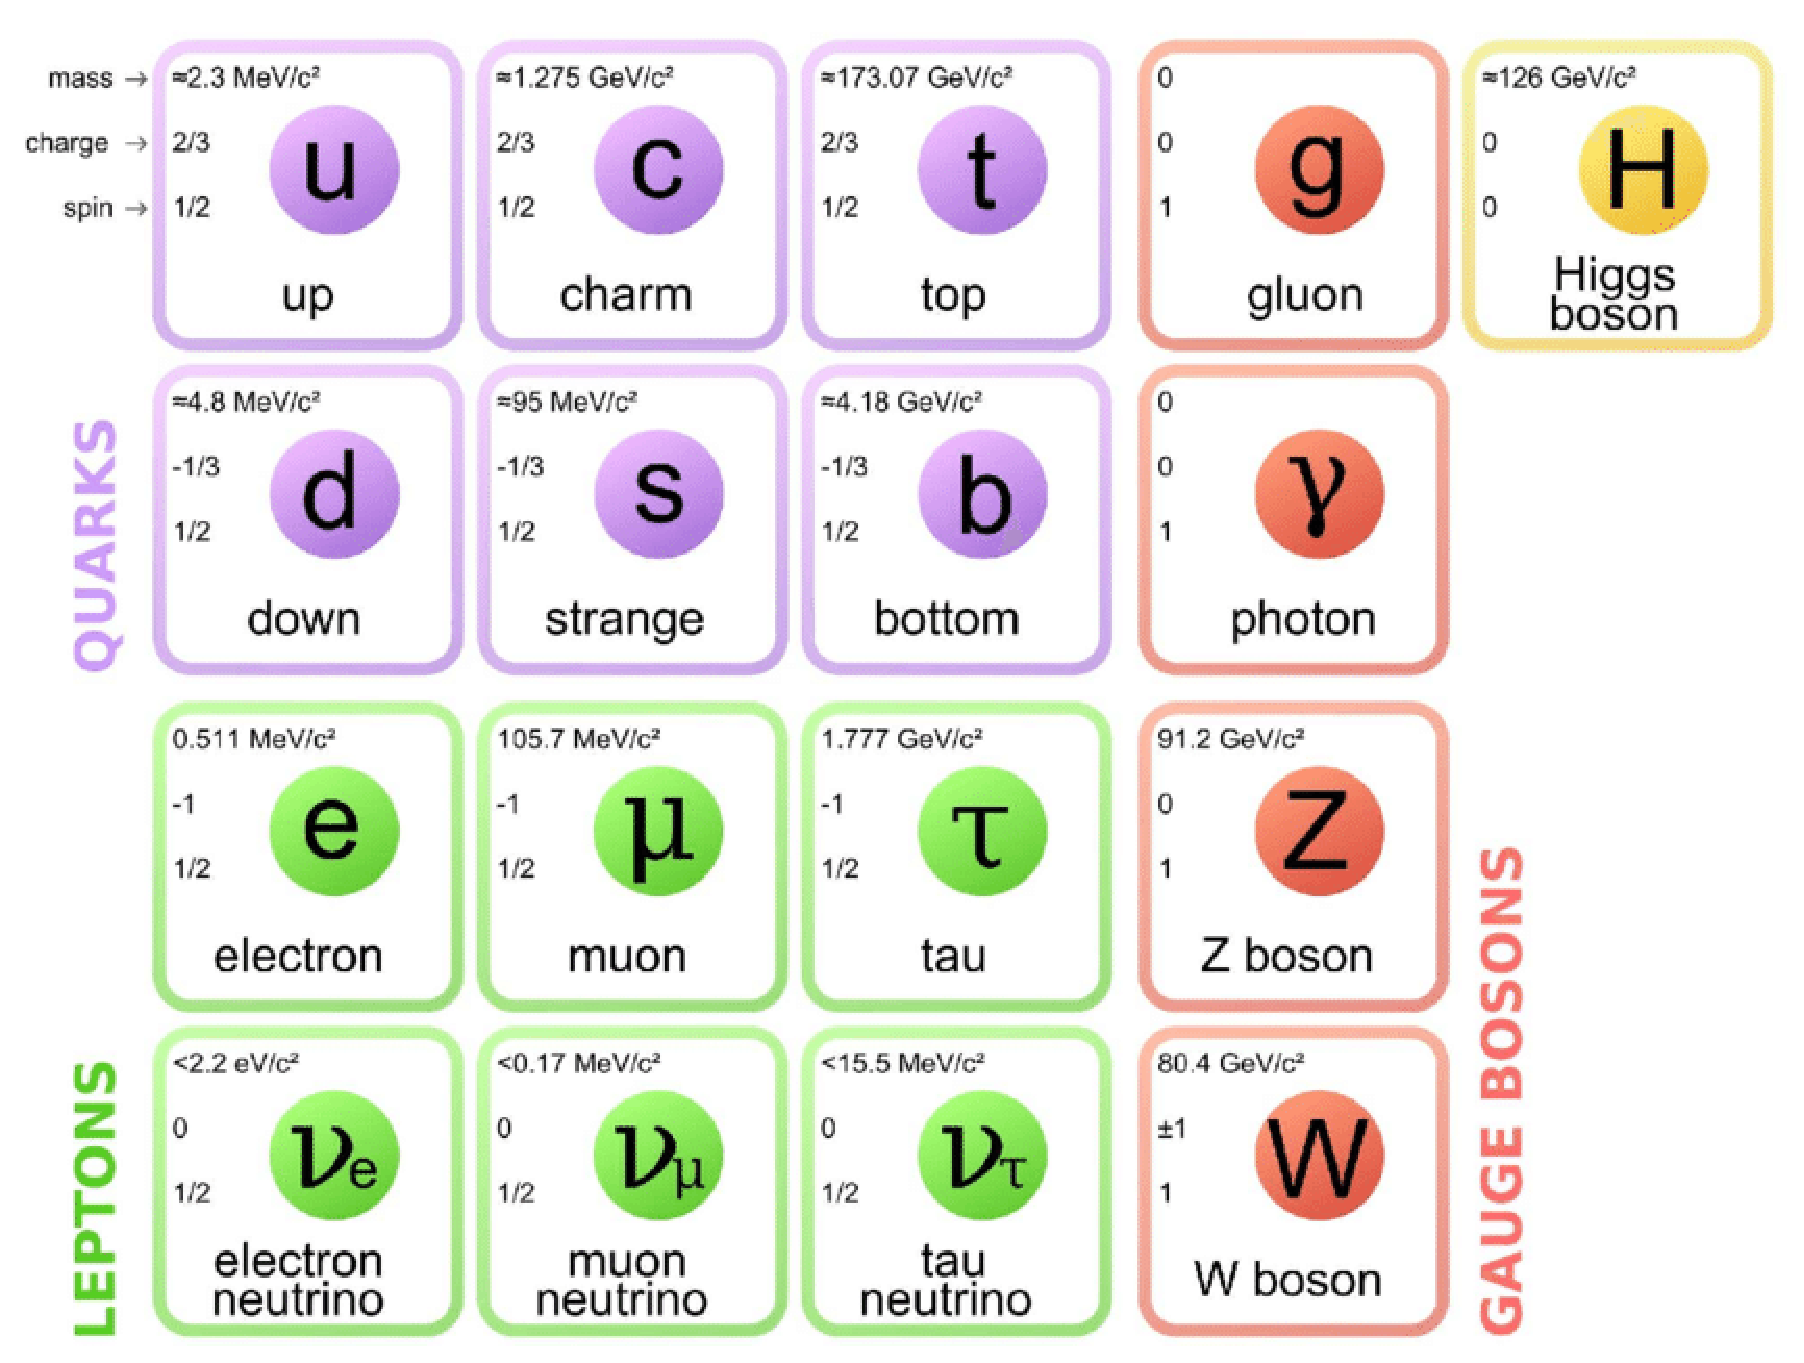
\includegraphics[scale=0.45]{Particle.eps}\\
		\caption{ The elementary particles of the SM  }
	\end{center}
\end{figure}

If an elementary particle carries the charge of a certain force, it is involved with the corresponding interaction. Quarks carry color charge (red, green, blue) and interact through the strong force mediated by massless gluons. The gluon has eight different states, which carrys a combination of color and anti-color charge in each state (color $SU(3)$ octet). The up, charm and top quarks carry a fractional electric charge of $2/3e$, while down, strange and bottom quarks carry a fractional electric charge of $-1/3e$. The charged leptons(electron, muon and tau) have an integer charge of $-e$. All electrically charged particles participate in the electromagnectic interaction mediated by the massless photon . Each charged lepton is paired with a neutral lepton (electron-, muon-, and tau-neutrino) with extremly low mass. All the particles participate in the weak interactions since they all carry an isospin, of which the $z$-compenent is either $+1/2$ (u, c, t-quark and neutrinos) or $-1/2$ (d, s, b-quark and charged leptons). The weak interactions are mediated by the neutral $Z$ or the electrically charged $W^{\pm}$ vector bosons. The masses of elementary particles in SM are acquired thorough the interactions with Higgs fields. 

In this chapter, we aim to give a brief introduction of the standard model of electroweak interactions\cite{H.P.PhyRep, BFLWQFT2, CQ}. We will introduce gauge invariance first. The spontaneous symmetry breaking and Higgs mechanism will be discussed next. Last we will review the contruction for the Lagragnian of the electroweak interactions.   


\section{Gauge Invariance}
\subsection{Abelian gauge invariance: Quantum electrodynamics}
Gauge theories are built with internal symmetries. For example, consider the $U(1)$ group of phase transformations of a free massive fermion field $\psi(x)$:
\begin{equation}
\psi(x)\to e^{-i\alpha}\psi(x),
\end{equation}
where $\alpha$ is an arbitrary phase parameter. The corresponding Lagranian density 
\begin{equation}
L(x)=\bar{\psi}(x)(i\slashed{\partial}-m)\psi(x)
\end{equation}
is invariant under these transformations. According to the N$\ddot{o}$ther theorem, this symmetry leads to a conserved current, 
\begin{eqnarray}
j_{\mu}(x)=\bar{\psi}(x)\gamma_\mu\psi(x),\hspace{2pt}
\partial^{\mu}j_\mu = 0.
\end{eqnarray}

The conserved charge,namely, generator of the $U(1)$ symmetry group, can be written as an integral over the charge density:
\begin{equation}
Q=\int d^3 x j_0(x).
\end{equation}

The invariance of the Lagragnian (1.2) under phase rotation indicates that the phase parameter $\alpha$ has no physical significance so that it could be chosen arbitrarily. It is unnatural to select a uniquely fixed $\alpha$ over all of the space-time, and it would be more natural to choose $\alpha$ locally, 
\begin{equation}
\psi(x)\to e^{-i\alpha(x)}\psi(x),
\end{equation}
where $\alpha$ depends on space-time in an arbitrary way. However, this modification brings a new problem. The Lagrangian (1.2) is no more invariant under the local phase rotations (1.5), because the derivative $\partial_\mu\psi(x)$ is transformed under phase rotation (1.5) by
\begin{equation}
\partial_\mu \psi(x)\to e^{-i\alpha(x)}\partial_\mu \psi(x)-ie^{i\alpha(x)}\partial_\mu\alpha(x)\psi(x).
\end{equation}
To solve this problem, We need to introduce a covariant derivative $D_\mu$, which has the property that $D\psi$ transforms under phase rotations like $\psi$:
\begin{equation}
D_\mu\psi(x)\to e^{-i\alpha(x)}D_\mu\psi(x).
\end{equation}

Such a covariant derivative can only be introduced if there exists another field, a vector field $A_\mu$ which interacts with the spinor field $\psi$. The covariant derivative $D_\mu$ is chosen as 
\begin{equation}
D_\mu=\partial_\mu + igA_\mu
\end{equation}
where $g$ is an arbitrary coupling constant, and $A_\mu$ transforms under a local phase transformation (gauge transformation) as follows:
\begin{equation}
A_\mu(x)\to A_\mu (x)+\frac{1}{g}\partial_\mu\alpha(x).
\end{equation}

We could easily verify that covariant (1.8) satisfies the requirement (1.7). Thus the invariance of the Lagrangian (1.2) under gauge transformations is recovered after replacing $\partial_\mu$ with $D_\mu$. However, we must add the kinetic term of the $A_\mu$ field for consistency, which must be gauge invariant in itself (only involving the gauge-invariant field strength).
\begin{equation}
F_{\mu\nu}=\partial_\nu A_\mu -\partial_\mu A_\nu.
\end{equation}

Therefore we obtain the Lagrangian which is invariant under gauge transformation
\begin{equation}
L=\bar{\psi}(i\slashed{D}-m)\psi-\frac{1}{4}F_{\mu\nu}F^{\mu\nu}.
\end{equation}
If we identify the spinor field $\psi$ with electron field, the vector field $A_\mu$ with photon field and replace $g$ by $e$ (electric charge), we obtain the Lagrangian for quantum electrodynamics (QED). Note that only the minimal coupling of the photon field to the electron field of the type $e\bar{\psi}\gamma_\mu\psi A^\mu$ is allowed due to the requirement of local gauge invariance. Furthermore a mass term for the photon filed of the type $m^2A_\mu A^\mu$ is forbidden to arise in the Lagrangian. 

\subsection{Non-Abelian gauge invariance}

The idea of non-Abelian gauge theories was formulated by Yang and Mills\cite{YM1954} in 1954. We successfully constructed the QED Lagrangian by imposing the local gauge invariance, $U(1$). This success encourages us to extend the gauge symmetry from an Abelian gauge case to a non-Abelian case. We will take the isospin symmetry as an example to formulate of the Non-Abelian gauge theories. The Lagrangian for the free protons and neutrons is 
\begin{equation}
L=\bar{N}(i\slashed{\partial}-m)N
\end{equation}
where $N$ represents the isospinor $(p,n)^T$. It is invariant under $SU(2)$ transformations
\begin{equation}
N\to e^{-i\alpha\sigma/2}N
\end{equation}
where $\sigma=(\sigma_1,\sigma_2,\sigma_3)$ ($\sigma\equiv$ Pauli matrices). and $\alpha$ is an arbitrary phase vector. The isotropic spin currents $\bar{N}\gamma_\mu\frac{1}{2}\sigma_iN$ are conserved. And the associated charges $T_i = \int d^3x \bar{N}\gamma\frac{1}{2}\sigma_iN$ generate the algebra of $SU(2)$:
\begin{equation}
[T_i, T_j] = i\epsilon_{ijk}T_k.
\end{equation} 
Note that the gauge transformations involving nondiagonal Pauli matrices $\sigma_1$, $\sigma_2$ result in the mixing between $p$ and $n$ states. However, this would not be a problem, since there would be no physical difference between proton and neutron for the isospin symmetry. Our selection for $p$ or $n$ totally depends on convention. Therefore it would be natural to redefine $p$ and $n$ locally in an arbitrary way, namely, we require the invariance under non-Abelian gauge transformations:
\begin{equation}
\binom{p}{n}\to e^{-i\alpha(x)\sigma/2}\binom{p}{n}
\end{equation} 
where $\alpha(x)$ is an arbitrary spacetime dependent phase vector. We will encounter the same problem as in the Abelian case discussed above: the derivative $\partial_\mu N$ which occurs in the Lagrangian (1.12) will not transform under local gauge transformations as $N$ itself, and we have to define a proper covariant derivative. To achieve this goal, we introduce a triplet of vector gauge fields $W_\mu^i$, which transforms under an infinitesimal gauge transformation as follows:
\begin{equation}
W_\mu^i\to W_\mu^i + \epsilon_{ijk}\alpha^j W_\mu^k+\frac{1}{g}\partial_\mu\alpha^i
\end{equation}
This transformation is analogous to eq. (1.9). The second term shows the local rotation of the $W^i$ in the isotropic space. The covariant derivative is defined as
\begin{equation}
D_\mu = \partial_\mu + igW_\mu
\end{equation}
where  $W_\mu=\frac{1}{2}\sigma W_\mu$. The Lagrangian of the system is 
\begin{equation}
L=\bar{N}(i\slashed{\partial}-m)N-\frac{1}{4}G_{\mu\nu}^i G_i^{\mu\nu},
\end{equation} 
where the $G_{\mu\nu}^i$ are the field strength tensors of the vector fields:
\begin{equation}
G_{\mu\nu}^i = \partial_\nu W_\mu^i - \partial_\mu W_\nu^i -g\epsilon^{ijk} W_{j\nu}W_{k\mu}
\end{equation}

This approach can be generalized to the case where an arbitrary gauge group and an arbitrary fermion representation are involved. The only changes are as follows:

(a) Replace the isospin matrices $\sigma$ with the corresponding matrices describing the transformation properties of the fermions under the gauge group.

(b) Replace $\epsilon_{ijk}$ with the structure constants $f_{ijk}$ of the gauge group. 

Note that the fermions can transform as an arbitrary representation of the gauge group, while the vector gauge fields must transform according to the adjoint representation. In the non-Abelian gauge theory, the vector fields interact with each other directly ("they are charged"). This is not the case in the Abelian theory where the vector field is neutral. The Lagrangian of the non-Abelian gauge theory (1.18) describes the interactions of massive fermions with massless gauge bosons.


\section{Spontaneous Symmetry Breaking}
It is known that the weak interactions are mediated by massive vector bosons $Z$ and $W^{\pm}$. However, we have seen above that the non-Abelian gauge invariance requires the gauge bosons to be massless. This means we must seek another possibility to introduce masses for the gauge fields in a more subtle way, such that the local gauge invariance is preserved. This can be realized by generating the gauge boson masses via a spotaneous breaking of the gauge symmetry. 

Usually the equations of motion for a physical system are symmetric under some symmetry transformations, however, the ground state of the systems is not. For example, the Hamiltonian for an infinitely extended ferromagnet is invariant under rotations in space. However, the ground state breaks the rotational symmetry since the individual spins are always aligned in an arbitrary direction. Similar situations arise in the field theory often, and we will discuss several examples of spontaneous breaking field theories.

The simplest example to exhibit the phenomenon of spontaneous symmetry breaking is the $\phi^4$ theory. Consider the Lagrangian
\begin{equation}
L=\frac{1}{2}(\partial^\mu \phi\partial_\mu \phi)-\frac{1}{2}\mu^2\phi^2-\frac{1}{4}\lambda\phi^4.
\end{equation}
The Lagrangian (1.20) is invariant under the parity transformation $P$, defined by $\phi\stackrel{P}{\to} -\phi$. The ground state (vacuum state $\Ket{0}$) of the theory is the one where $\phi$ vanishes everywhere. It is invariant under the parity transformation: $P\Ket{0}=\Ket{0}$. 

\begin{figure}
	\begin{center}
		\includegraphics[scale=0.08]{index.eps}\\
		\caption{The potential V($\phi$) of the scalar field $\phi$ in the case $\mu^2>0$ (left) and $\mu^2>0$ (right)  }
	\end{center}
\end{figure}

If the parameter $\mu^2>0$, the potential $V(\phi)=\frac{1}{2}\mu^2\phi^2+\frac{1}{4}\lambda\phi^4$ has a unique minimum at $\phi=0$, as shown in Figure 1.2, which corresponds to the vacuum state. 

If the parameter $\mu^2>0$, the situation is that of a spontaneously broken symmetry. The potential 
\begin{equation}
V(\phi)=-\frac{1}{2}|\mu^2|\phi^2+\frac{1}{4}|\lambda|\phi^4,
\end{equation}
shown in Figure 1.2, has minima at 
\begin{equation}
\Bra{0}\phi\Ket{0} = \pm\sqrt{-\mu^2/|\lambda|}\equiv \pm v,
\end{equation}
which corresponds to two possible ground states. These vacuums are not invariant under parity transformation since $v \neq -v$. Thus the parity invariance is spontaneously broken. It is useful to define a new field $\phi'$, for which $\Bra{0}\phi'\Ket{0}$=0, i.e. $\phi'=\phi-v$. In terms of $\phi$ we have 
\begin{equation}
L=\frac{1}{2}(\partial^\mu \phi'\partial_\mu \phi')-\mu^2\phi'^2-\frac{1}{4}\lambda\phi'^4-\lambda v\phi^3+\text{const}.
\end{equation}

We see that the Lagrangian (1.20) with $\mu^2<0$ describes self-interacting scalar particles with mass $\sqrt{2}|\mu|$. 




Next, let us consider the theory of a complex scalar field $\phi =\frac{\sqrt{2}}{2}(\phi_1+i\phi_2)$. Consider the Lagrangian
\begin{align}
L&=\frac{1}{2}(\partial^\mu \phi^{\ast} \partial_\mu \phi)-\frac{1}{2}\mu^2\phi^2-\frac{1}{4}\lambda\phi^4\nonumber\\
&=\frac{1}{2}\partial^\mu\phi_1\partial_\mu\phi_1+\frac{1}{2}\partial^\mu\phi_2\partial_\mu\phi_2-\frac{1}{2}\mu^2(\phi_1^2+\phi_2^2)-\frac{1}{4}\lambda(\phi_1^2+\phi_2^2)^2.
\end{align}

It is invariant under the phase transformation $\phi \to e^{-i\theta}\phi$. For $\mu^2>0$ this Lagrangian describes a self-interacting scalar complex field of mass $\mu$. 

Assume we choose $\mu^2<0$ now, then the potential $V(\phi)$ has a minimum at $(\phi_1^2+\phi_2^2)=2|\phi|^2=-\mu^2/\lambda$. So the minimum of the potential occurs along a circle of radius $\sqrt{-\mu^2/\lambda}$ around the origin. Because we could pick any point on the circle as the vacuum state, we are now dealing with an infinite number of possible vacua. Let us take an arbitrary point on the circle as the vacuum, described by the coordinates $v=(v_1,v_2)$. Since the Lagrangian is invariant under phase transformations, we could let this point lie on the 
positive real axis, namely, $v=(\sqrt{-\mu^2/\lambda})$, which implies $\Bra{0}\phi_1\Ket{0}=\sqrt{-\mu^2/\lambda}$, $\Bra{0}\phi_2\Ket{0}=0$.

Now we define $\phi_1'=\phi_1-\Bra{0}\phi_1\Ket{0}$, then the Lagrangian (1.24) becomes
\begin{equation}
L=\frac{1}{2}\partial^\mu\phi'_1\partial_\mu\phi'_1+\frac{1}{2}\partial^\mu\phi_2\partial_\mu\phi_2+\mu^2{\phi'_1}^2-\frac{1}{2}\lambda v\phi'_1({\phi'_1}^2+{\phi_2}^2)-\frac{\lambda}{4}({\phi'_1}^2+{\phi_2}^2)^2,
\end{equation}
where $v=\sqrt{-\mu^2/\lambda}$. From the Lagrangian (1.25), we see that the field $\phi_1$ describes a particle of mass $\sqrt{2|\mu|}$, but $\phi_2$ is still massless.

The system described above gives an example of the Goldstone theorem \cite{Nambu,NambuLasinio1,NambuLasinio2,Goldstone,Bludman}: for every spontaneously broken continuous symmetry, the theory contains massless Goldstone bosons (spin-$0$).

The example discussed above exhibits an invariance under the global gauge group $U(1)$ which is isomorphic to $O(2)$. It could be generalized to involve the gauge group $O(n)$. Let us consider the Lagrangian
\begin{eqnarray}
&&L=\frac{1}{2}(\partial^\mu \phi_i\partial_\mu \phi_i)-\frac{1}{2}\mu^2\phi_i\phi_i-\frac{1}{4}\lambda(\phi_i\phi_i)^2, i = 1,2,\cdots,n;\nonumber\\
&& \phi_i \equiv \text{real scalar field}; \text{ summation over $i$}.
\end{eqnarray}
This Lagrangian is invariant under the group $O(n)$. For $\mu^2<0$ the minimum of the potential is at $v=\sqrt{-\mu^2/\lambda}$. The potential $V(\phi)$ exhibits the minimum at $\phi_i\phi_i=-\mu^2/\lambda$, i.e. it arises on the $n$-dimensional sphere of radius $\sqrt{-\mu^2/\lambda}$ in the $n$-dimensional space defined by the fields $\phi_i$. Because of the $O(n)$-invariance of the Lagrangian we could select the coordinates of fields so that the vacuum expectation value of the field vector $\phi_i$ is defined as follows:
\begin{equation}
\bra{0}\phi\ket{0}=
\begin{bmatrix}
0\\0\\0\\\vdots\\0\\v
\end{bmatrix}.
\end{equation}

Note that the first $(n-1)$ components of $\bra{0}\phi\ket{0}$ are zero, the vacuum remains invariant under the subgroup $O(n-1)$. We see that the vacuum expectation value $\bra{0}\phi\ket{0}$ breaks the $O(n)$-invariance in a particular way. Let us see the point (1.27) in the n-dimensional space of the fields $\phi_i$. There are $(n-1)$ linearly independent directions to leave this point, but to stay on the sphere which minimizes the potential. Therefore there must exist $(n-1)$ massless Goldstone bosons, according to the Goldstone theorem. So the Lagrangian (1.26) describes a massive field of mass $\sqrt{-2\mu^2}$ and $(n-1)$ massless Goldstone bosons.

The group $O(n)$ has $\frac{1}{2}n(n-1)$ generators, while the subgroup $O(n-1)$ has $\frac{1}{2}(n-1)(n-2)$ generators. This means $(n-1)$ generators of $O(n)$ do not leave the vacuum invariant. On the other hand, we have $(n-1)$ massless Goldstone bosons, namely, the number of massless Goldstone bosons is equal to the number of generators which are broken spontaneously. This feature is a special property of the $O(n)$ model we have discussed above, but a general feature of spontaneously broken theories involving scalar fields. The number of Goldstone bosons corresponds always to the number of the spontaneously broken generators as a consequence of the general Goldstone theorem\cite{AbersLee}.
\newpage
\section{The Higgs Mechanism}
As we discussed above, the local gauge invariance requires gauge bosons to be massless only. However, in reality, the observed gauge bosons of weak interactions $Z$ and $W^{\pm}$ are massive. In order to reconcile this contradiction, we need to incorporate Higgs mechanism\cite{Higgs1,Higgs2,Higgs3} into the gauge theory, by which spontaneous symmetry breaking generates a mass for a gauge boson. 

\subsection{The Higgs Mechanism in the Abelian Theory}
Let us consider the Lagrangian 
\begin{equation}
L=\partial^\mu \phi^{\ast}\partial_\mu\phi-\mu^2\phi^{\ast}\phi-\lambda(\phi^{\ast}\phi)^2,
\end{equation}
which is invariant under the global gauge transformations $\phi\to e^{-i\alpha}\phi$, i.e., $U(1)$ gauge group. However, we need invariance under the local gauge transformations $\phi\to e^{-i\alpha(x)}\phi$. In order to achieve this goal, we need to introduce a gauge field $A_\mu$. Repeating the procedure outlined in Subsection 1.1.1, we arrive at 
\begin{equation}
L=(D^\mu \phi)^{\ast}D_\mu\phi-\mu^2\phi^{\ast}\phi-\lambda(\phi^{\ast}\phi)^2-\frac{1}{4}F_{\mu\nu}F^{\mu\nu},
\end{equation}
where $F_{\mu\nu}=\partial_\nu A_\mu - \partial_\mu A_\nu$, and $D_\mu=\partial_\mu+igA_\mu$.

We note that the various fields transform under local gauge transformations as follows:
\begin{eqnarray}
&&\phi(x)\to e^{-i\alpha(x)}\phi(x),\nonumber\\
&&A_\mu (x)\to A_\nu (x)+\frac{1}{g}\partial_\mu\alpha(x).
\end{eqnarray}

For $\mu^2>0$ the Lagrangian (1.29) describes the system of a massive scalar field, coupled to a massless gauge field $A_\mu$. If we let $g=e$(electric charge), then we are dealing with the scalar electrodynamics.  

For $\mu^2<0$ the gauge symmetry is spontaneously broken, as discussed in Section 1.2. We have known that the Lagrangian (1.28) describes a massive scalar field, accompanied by a massless Goldstone by following the approach outlined in section 1.2. Next, we will investigate what will happen in case of the  gauge invariant Lagrangian (1.29). Let us make the substitution
\begin{equation}
\phi_1=\phi'_1+\bra{0}\phi_1\ket{0}=\phi_1+v, v=\sqrt{-\mu^2/\lambda}
\end{equation} 
in eq. (1.29). We therefore expand the scalar field $\phi(x)$ around the vacuum expectation value $\bra{0}\phi\ket{0}$ and arrive at
\begin{equation}
L=-\frac{1}{4}F_{\mu\nu}F^{\mu\nu}+\frac{1}{2}\partial^\mu \phi_1\partial_\mu\phi_1+\frac{1}{2}\partial^\mu \phi_2\partial_\mu\phi_2+\frac{1}{2}g^2v^2 A_\mu A^\mu - gvA_\mu\partial^\mu\phi_2.
\end{equation}

We find that following new terms arise:
\begin{equation}
\frac{1}{2}g^2v^2 A_\mu A^\mu,
\end{equation}
\begin{equation}
 - gvA_\mu\partial^\mu\phi_2.
\end{equation}
The term (1.33) could be interpreted as the gauge boson mass term where the mass $m_A^2 = g^2v^2$ arises from the nonvanishing vacuum expectation value of $\phi$. However, the interpretation of the term (1.34) is sort of vague, since it mixes the gauge field with the Goldstone boson $\phi$. In order to clarify this condition, let us consider the gauge transformation $\phi\to e^{-i\alpha}\phi$ in terms of $\phi'_1$ and $\phi_2$.

For an infinitesimal parameter $\alpha$ we have
\begin{eqnarray}
&&\phi\to(1-i\alpha)\phi,\nonumber\\
&&\phi_1\to\phi_1-\alpha\phi_2,\nonumber\\
&&\phi_2\to\phi_2+\alpha\phi_1,
\end{eqnarray}
and we find
\begin{eqnarray}
&&\phi'_1\to\phi'_1-\alpha\phi_2,\nonumber\\
&&\phi_2\to\phi_2+\alpha v+\alpha\phi'_1,
\end{eqnarray}

Thus $\phi_2$ undergoes an inhomogenous gauge transformation like the gauge field $A_\mu$. So we could use the freedom of gauge to set $\phi_2=0$, in which the mixing term (1.34) and the Goldstone boson vanish. 

As we see, the introduction of the gauge field $A_\mu$ and the requirement of local gauge invariance fully change the physical condition: the Lagrangian (1.28) describes a massive scalar field accompanied with a massless Goldstone boson, while the Lagrangian (1.29) describes a massive gauge boson $A_\mu$ and a massive scalar boson $\phi$. However, the total number of the particle states remains unchanged. Before spontaneous symmetry breaking, the theory had four particle states: two spin-zero particles $\phi$ and $\phi^{\ast}$ plus two polarization states of the massless gauge boson $A_\mu$, i.e. four states in total. After spontaneous symmetry breaking, we have one scalar particle plus three polarization states of the massive gauge boson $A_\mu$, i.e. still four states. Therefore, we could say that the massless gauge boson "ate" the massless Goldstone boson to become a massive gauge boson. 


The Higgs mechanism introduced above is important for the following discussion. In general theories involving massive gauge bosons are non-renormalizable, because of the $k_\mu k_\nu/m^2$-term in the gauge boson propagator. However, in the original Lagrangian (1.29), the gauge field is formally massless, where no issues with renormalizability occurs. It turns out that spontaneous symmetry breaking would not affect the renormalizibility of the theory\cite{thooft1,thooft2,tHooftVeltman}. Note that for the Abelian gauge theory described by the Lagrangian (1.28), the spontaneous generation of the gauge boson mass is not necessary to achieve renormalizability. We would not undermine the renormalizablity if we introduce a mass term for the gauge boson, provided that the gauge field $A_\mu$ is coupled with a conserved current. However, this is not valid for a non-Abelian theory. The spontaneous generation of gauge boson masses is the only way to ensure renormalizability.

In sum, Higgs meachanism is a remarkable result, suggesting the possibility of establishing spontaneously broken gauge theories in which the interactions are mediated by massive gauge bosons. 
 

\subsection{The Higgs Mechanism in the non-Abelian Theory}
In order to explore additional complications from spontaneous symmetry breaking of a non-Abelian theory, we choose $SU(2)$ gauge theory as a prototype.

At first, we choose a doublet representation of complex scalar fields, coupled to the gauge fields in a gauge invariant way. Such a Lagrangian is defined by
\begin{equation}
L=-\frac{1}{4}G^i_{\mu\nu}G_i^{\mu\nu}+\Big(\partial^\mu\phi+i\frac{g}{2}\sigma^iB^{\mu i}\phi\Big)^{\dagger}
\Big(\partial_\mu\phi+i\frac{g}{2}\sigma_i B_{\mu}^i\phi\Big)-\mu^2\phi^{\dagger}\phi-\lambda(\phi^{\dagger}\phi)^2,
\end{equation}
where the scalar field $\phi$ represents the $SU(2)$ doublet
\begin{equation}
\phi=\binom{\phi_a}{\phi_b},
\end{equation}
and the $\sigma_i$'s denote the Pauli matrices.

For $\mu^2>0$ the Lagrangian (1.37) describes a system of massless gauge fields in interaction with massive scalars of mass $\mu$. Now suppose we choose $\mu^2<0$, then  the potential $V(\phi)=\mu^2\phi^\dagger\phi+\lambda(\phi^\dagger\phi)^2$ exhibits its minimum at finite values of $\phi$. The manifold of points in the space of fields $\phi_a$, $\phi_b$ for which the minimum of the potential $V(\phi)$ occurs is invariant under $SU(2)$-transformations. Therefore, we could choose a specific $SU(2)$ frame for which we have $\bra{0}\phi\ket{0}=\frac{1}{\sqrt{2}}\binom{0}{v}$, where $v=\sqrt{-\mu^2/\lambda}$. Form eq. (2.35) we obtain the mass term of the gauge field, which is
\begin{align}
\frac{g^2}{4}[(\sigma^i B^i_\mu)]^{\dagger}[(\sigma^i B^i_\mu)]&=\frac{g^2}{4}(\phi^\dagger\tau^j\tau^i\phi)(B_\mu^i B^{\mu i})\nonumber\\
&=\frac{g^2}{8}\cdot v^2[(B^1_\mu)^2+(B^2_\mu)^2+(B^3_\mu)^2].
\end{align}

Thus we could conclude: we obtain massive gauge fields after spontaneous symmetry breaking. The gauge boson mass matrix is $SU(2)$ symmetric, namely, the three gauge bosons are degenerate in mass. This is a special feature of the spontaneous symmetry breaking involving an $SU(2)$ doublet.

Note that the particle content of the theory includes three massive gauge fields and one massive scalar field. Three of the scalar fields (four real fields originally) have been eaten to provide the longitudinal components of the massive gauge fields. 

Next, we choose an $SU(2)$ triplet representation of real scalar fields
\begin{equation}
\phi=\left(
\begin{array}{c}
\phi_1\\ \phi_2\\ \phi_3
\end{array}
\right).
\end{equation}
We require invariance under the gauge transformation
\begin{equation}
\phi\to e^{iT_i \alpha_i}\phi,
\end{equation}
where the exponential factor is a $3\times3$ matrix. The operator $T_i$ generates isospin rotations about the $i$-axis and satisfies the usual $SU(2)$ algebra
\begin{equation}
[T^j,T^k]=i\epsilon_{jkl}T^l.
\end{equation}
The explicit matrix representation is 
\begin{equation}
(T^j)_{kl} = -i\epsilon_{jkl}.
\end{equation}

Following the procedure outline in Section 1.2, we have the covariant derivative as follows
\begin{equation}
D_\mu = \partial_\mu - igT_i B_{\mu i},
\end{equation}
or, in the ajoint representation, the covariant derivative takes the form,
\begin{equation}
(D_\mu)_{kl}=\delta_{kl}\partial_\mu + g\epsilon_{jkl}B_{\mu j}.
\end{equation}
Then the Lagrangian of the theory is 
\begin{equation}
L=-\frac{1}{4}G^i_{\mu\nu}G_i^{\mu\nu}+\frac{1}{2}(\partial^\mu\phi_i-g\epsilon_{ijk}B^\mu_j\phi_k)
(\partial_\mu\phi_i-g\epsilon_{ilm}B^\mu_l\phi_m)-\frac{1}{2}\mu^2\phi_i\phi_i-\frac{1}{4}\lambda(\phi_i\phi_i)^2.
\end{equation}

When $\phi$ is the unique minima of the potential $V(\phi)=\frac{1}{2}\mu^2\phi_i\phi_i+\frac{1}{4}\lambda(\phi_i\phi_i)^2$, the spectrum is that of an ordinary, isospin-conserving gauge filed theory: three massive scalar fields, each with mass $\mu$, and three massless gauge fields $B_\mu$. Since each massless gauge boson has two polarization states, then the number of particle states is $3\times1+3\times2=9$. 

If we choose $\mu^2<0$, spontaneous symmetry breaking occurs. We could choose a particular coordinate system of fields such that we have 
\begin{equation}
\bra{0}\phi\ket{0}=\left(
\begin{array}{c}
0\\0\\v
\end{array}\right).
\end{equation} 

This vector remains invariant under rotation generated by $T_3$, i.e. the subgroup $U(1)\subset SU(2)$, generated by the third generator $T_3$ remains unbroken.

We shift the scalar fields and expand around the $v$, using 
\begin{eqnarray}
\phi \to \exp\biggl[\frac{i}{v}(\zeta_1 T_1+\zeta_2 T_2)  \biggr]
\left(
\begin{array}{c}
	0\\0\\v+\eta
\end{array}
\right).
\end{eqnarray}

We could exploit the gauge invariance of the theory by letting
\begin{eqnarray}
\phi \to \exp\biggl[-\frac{i}{v}(\zeta_1 T_1+\zeta_2 T_2)  \biggr]
\phi=\left(
\begin{array}{c}
0\\0\\v+\eta
\end{array}
\right).
\end{eqnarray}
With the help of the new gauge, we obtain the Lagrangian
\begin{equation}
L=\frac{1}{2}(\partial_\mu\eta\partial^\mu\eta+2\mu^2\eta^2)-\frac{1}{4}G_{\mu\nu}^i G^{\mu\nu i}+\frac{1}{2}g^2v^2[B^1_\mu B^{1\mu}+B^2_\mu B^{2\mu}]+\cdots
\end{equation}

From this Lagrangian, we conclude: $\eta$ has become a massive Higgs scalar field, with mass $\sqrt{-2\mu^2}$; the Goldstone bosons $\eta_1$ and $\eta_2$ have disappeared completely, i.e., they have been eaten up by gauge fields; the gauge bosons $B^{\mu}_1$ and $B^\mu_2$ respective coupled to the broken generators $T_1$ and $T_2$ have acquired a common mass $gv$; the gauge boson $B^\mu_3$ remains massless, reflecting the invariance of the vacuum under the generator $T_3$.


\section{Standard Model of the electroweak interactions}
\subsection{The General Ideas for Building Spontaneous Broken Gauge Theories }
After investigating the examples above, we are ready to discuss the general features of spontaneous broken gauge theories. Let us consider a Lagrangian which is invariant under local gauge transformations of a group $G$. The generatos $T_i$ follow the commutation relations
\begin{equation}
[T_i, T_j]=if_{ijk}T_k,
\end{equation}
where $i,j,k = 1,\cdots,N$ and $f_{ijk}$ is the structure constant of $G$. An arbitrary infinitesimal transformation of the group $G$ could be parametrized by $1-i\epsilon_i T_i$, where $\epsilon_i$'s are infinitesimal parameters.

The scalar field $\phi$ is assumed to transform under a $n$-dimensional representation of G. We assume that the field $\phi$ are real, since a complex field $\phi$ can always be decomposed into two real ones. For an infinitesimal transformation of $G$ we have:
\begin{equation}
\delta \phi=i\epsilon_i S_i\phi.
\end{equation}
The Lagrangian is defined by
\begin{equation}
L=-\frac{1}{4}G^i_{\mu\nu}G_i^{\mu\nu}+\frac{1}{2}[(\partial^\mu +igS_iA_i^\mu)\phi]^{\dagger}[(\partial_\mu +igS_jA_{j\mu})\phi]-V(\phi),
\end{equation}
where $V(\phi)$ is a quartic potential in $\phi$, invariant under $G$.

We assume that spontaneous symmetry breaking occurs and the potential exhibits its minimum at $\phi=v$, where $v$ is a $n$-dimensional vector. The gauge boson mass matrix is then given by 
\begin{equation}
(M^2)_{ij}=-g^2(S_i v)\cdot (S_j v).
\end{equation}

In general, there will exist a $M$-dimensional subgroup $G'$ of $G$, which preserves an invariance of the vacuum. 

Let $T_i(G')$ be the generators of $G'$, then $T_i(G')v=S_i(G')v=0$. There exist $(N-M)$ generators of $G$, for which $T_i v\ne0$, i.e. one has $(N-M)$ Goldstone bosons. Therefore the $N\times N$ dimensional mass matrix denoted in eq.(1.54) is actually an $(N-M)\times(N-M)$ dimensional matrix, if we leave out all terms for which $S_i v=0$ because of the $S$-invariance of the vacuum. The mass matrix (1.54) needs to be diagonalized if we would like to find the massive vector bosons of definite mass. There exist $(N-M)$ massive gauge bosons. The $(N-M)$ Goldstone bosons are aborbed into the longitudinal components of the $(N-M)$ massive gauge bosons.   

Up to now, our discussion mainly focuses on scalar and vector fields. Next, we need to incorporate fermion fields into the gauge theory, by adding to the Lagrangian (1.53) the terms
\begin{equation}
L^{\text{fermion}}=\bar{\psi}_L(i\slashed{\partial}-gf_{Li}\slashed{A}_i)
\psi_L+\bar{\psi}_R(i\slashed{\partial}-gf_{Ri}\slashed{A}_i)
\psi_R-(m\bar{\psi}_R\psi_L+\text{h.c.})
\end{equation} 
and
\begin{equation}
L^{\text{int}}=-G\bar{\psi}_R(R\phi)\psi_L+h.c.
\end{equation}
where $\psi_L$, $\psi_R$ stand for the left-handed and right-handed fermion fields. The fields $\psi_L$ and $\psi_R$ transform under G as certain irreducible representations. The matrices $f_L$, $f_R$ denote the transformation properties of the left-handed and right-handed fermion fields. In eq. (2.55), we include the Yukawa interaction term of the fermion fields with the scalar fields. The matrices $R$ are constructed so that $\bar{\psi}_R(R\phi)\bar{\psi}_L$ is invariant under the gauge group. We also include a bare mass term $(m\bar{\psi}_R\psi_L+h.c.)$, which must be $G$-invariant. 

From the eqs. (1.55) and (1.56) we obtain the fermion mass matrix after the spontaneous symmetry breaking,
\begin{equation}
L^{\text{fermion mass}}=-G\bar{\psi}_R(Rv)\psi_L-m\bar{\psi}_R\psi_L+h.c.
\end{equation}

After introducing the general properties of spontaneous broken gauge theories, we are ready to give the general recipe for building renormalizable gauge theories. The Lagrangian is constructed as follows:

1. Select the gauge group, the representations of left-handed and right-handed fermions and the scalar fields.

2. Couple the gauge fields invariantly to the fermion and scalar fields.

3. Couple the gauge invariant quartic polynomial of the scalar fields so that the potential reaches its minimum for nonvanishing vacuum expectation values $v$.

4. Construct the gauge invariant Yukawa couplings between the fermions and scalars.

The gauge boson mass matrix has the structure: 
$$
\frac{1}{2}g^2v^2W_\mu^2,
$$
the fermion mass matrix is
$$
G\cdot v\bar{\psi}\psi.
$$

\subsection{The Glashow-Weinberg-Salam Theory of Electroweak Interations}
We are now ready to write down the spontaneously broken gauge theory that gives experimentally confirmed description of weak and electromagnetic interactions, a model introduced by Glashow, Weinberg, and Salam (GWS) \cite{Glashow1961,Weinberg,Salam}. We begin with the doublet of the weak isospin consisting of left-handed electron and its neutrino,
\begin{equation}
\psi_{L}^e \equiv \binom{\nu_e}{e}_L,
\end{equation}
where the left-handed states are
\begin{align}
\nu_L&=\frac{1}{2}(1-\gamma_5)\nu_e\nonumber\\
e_L&=\frac{1}{2}(1-\gamma_5)e
\end{align}
The electron neutrino is known to be nearly massless. It is convenient to idealize it as exactly massless, in which case the right-handed state 
\begin{eqnarray}
\nu_R = \frac{1}{2}(1+\gamma_5)\nu_e
\end{eqnarray}
does not exist. Thus we have only one right-handed fermion,
\begin{equation}
\psi_R^e \equiv e_R =\frac{1}{2}(1+\gamma_5)e,
\end{equation}
which is an $SU(2)$-singlet.

Note that we need to have the $U(1)$-factor in the gauge group $SU(2)\otimes U(1)$ to represent the electric charge. This cannot be an $SU(2)$ generator since the photon couples both to the left-handed and right-handed electron. To incorporate the electromagnetic interaction, we denote the $U(1)$ generator as ``weak hypercharge", $Y$. Requiring that the Gell-Mann-Nishijima relation for electric charge,
\begin{equation}
Q=I_3+\frac{1}{2}Y
\end{equation}
be satisfied leads to the assignments
\begin{eqnarray}
&&Y_L =-1,\nonumber\\
&&Y_R = -2.
\end{eqnarray}
By construction, the weak-isopin projection $I_3$ and the weak hypercharge $Y$ commute:
\begin{equation}
[I_3,Y]=0.
\end{equation}
Let us take the group of transformations generated by $I$ and $Y$ to be the gauge group $SU(2)_L\otimes U(1)_Y$ for the gauge theory. In order to construct the theory, we introduce the gauge bosons $A_\mu^1$, $A_\mu^2$, $A_\mu^3$ for $SU(2)_L$ and $B_\mu$ for $U(1)_Y$.

The Lagrangian for the theory might be written as
\begin{equation}
L=L^{\text{gauge}}+L^{\text{fermion}}+L^{\text{scalar}},
\end{equation}
and the gauge boson part of the Lagrangian is
\begin{equation}
L^{\text{gauge}}=-\frac{1}{4}F^l_{\mu\nu}F_l^{\mu\nu}-\frac{1}{4}G_{\mu\nu}G^{\mu\nu}
\end{equation}
where 
\begin{equation}
F^l_{\mu\nu}=\partial_\nu A^l_\mu-\partial_\mu A^l_\nu+g\epsilon_{jkl} A^j_{\mu} A^k_{\nu}
\end{equation}
for the $SU(2)_L$ gauge fields and
\begin{equation}
G_{\mu\nu}=\partial_\nu B_\mu -\partial_\mu B_\nu
\end{equation}
for the $U(1)_Y$ gauge field. 

We introduce a complex doublet of scalar fields
\begin{eqnarray}
\phi\equiv\binom{\phi^{\dagger}}{\phi_0}
\end{eqnarray}
which transforms as an $SU(2)_L$ doublet and has the hypercharge 
\begin{equation*}
Y_\phi=1
\end{equation*}
by virtue of the Gell-Mann-Nishijima relation.

Now we are ready to write down the fermion and scalar parts of the Lagrangian:
\begin{equation}
L^{\text{fermion}}=\bar{\psi}_R^e\bigg(\slashed{\partial} +\frac{ig'}{2}\slashed{B}Y\bigg)\psi_R^e+\bar{\psi}_L^e i\bigg( \slashed{\partial}+\frac{ig'}{2}\slashed{B}Y+\frac{ig}{2}\sigma_i\slashed{A}_i  \bigg)\psi_{L}^e
\end{equation}
and 
\begin{equation}
L^{\text{scalar}}=(D^\mu \phi)^{\dagger}(D_\mu\phi)-V(\phi^{\dagger}\phi),
\end{equation}
where the covariant derivative is
\begin{equation}
D_\mu =\partial_\mu +\frac{ig'}{2}B_\mu Y +\frac{ig}{2}\sigma_i A_{i\mu }
\end{equation}
and the most general form of the potential is 
\begin{equation}
V(\phi^\dagger\phi)=\mu^2(\phi^\dagger\phi)+|\lambda|(\phi^\dagger\phi).
\end{equation}
We also add an interaction term, which involves Yukawa couplings of the scalar to the fermions,
\begin{equation}
L^{\text{Yukawa}}=-G_e [\bar{\psi}_R^e(\phi^\dagger\psi_{L}^e)+(\bar{\psi}_L^e)\psi_R^e],
\end{equation}
which is symmetric under $SU(2)_L\otimes U(1)_Y$ transformations,

Now let us take $\mu^2<0$, then the $SU(2)_L\otimes U(1)_Y$ symmetry is spontaneously broken.  We choose a $SU(2)$ frame so that the vacuum expectation values of $\phi$ take the form:
\begin{equation}
\bra{0}\phi\ket{0}=\binom{0}{v/\sqrt{2}},
\end{equation}
where $v=\sqrt{-\mu^2/|\lambda|}$, which breaks both $SU(2)_L$ and $U(1)_Y$ symmetries. However, the electric charge, which is a linear combination of $T_3$ and $Y$ remains unbroken. The photon will therefore remain massless, while three other gauge bosons will aquire mass.

We next expand the Lagrangian about the minimum of the Higgs potential $V$ by letting
\begin{equation}
\phi=\exp\bigg(\frac{i\zeta_i\sigma_i}{2v} \bigg)\binom{0}{(v+\eta)/\sqrt{2}}
\end{equation}
and transforming to U-gauge:
\begin{equation}
\phi\to \exp\bigg(-\frac{i\zeta_i\sigma_i}{2v} \bigg)\phi=\binom{0}{(v+\eta)/\sqrt{2}},
\end{equation}
\begin{equation}
\sigma_i A_{i\mu}\to \sigma_i A'_{i\mu},
\end{equation}
\begin{equation}
B_\mu \to B_\mu,
\end{equation}
\begin{equation}
\psi_R^e \to \psi_R^e,
\end{equation}
\begin{equation}
\psi_L \to \exp\bigg(-\frac{i\zeta_i\sigma_i}{2v} \bigg)
\end{equation}

We now express the Lagrangian in terms of the U-gauge fields (1.77-1.81) and explore the results of spontaneous symmetry breaking. The Yukawa part of Lagrangian has become
\begin{eqnarray}
L^\text{Yukawa} = -G_e\frac{v+\eta}{\sqrt{2}}(\bar{e}_R e_L+\bar{e}_L e_R)=-\frac{G_e v}{\sqrt{2}}\bar{e}e-\frac{G_e \eta}{\sqrt{2}}\bar{e}e
\end{eqnarray}
so the electron has aquired a mass
\begin{equation}
m_e = G_e v/\sqrt{2}
\end{equation}

The scalar part of the Lagrangian now becomes
\begin{equation}
L^\text{scalar} =\frac{1}{2}(\partial^\mu\eta)(\partial_\mu\eta)-\mu^2\eta^2+\frac{v^2}{8}[g^2|A^1_\mu-iA^2_\mu|^2+(g'B_\mu-gA_\mu^3)^2]+\cdots
\end{equation}
We see immediately that the $\eta$ field has acquired a mass $m_H=\sqrt{-2\mu^2}$; it is the physical Higgs boson. If we define the charged gauge fields
\begin{equation}
W_\mu^\pm\equiv \frac{A_\mu^1\mp A_\mu^2}{\sqrt{2}},
\end{equation}
the term proportional to $g^2 v^2$ is identified as a mass term for the charge gauge bosons:
\begin{equation}
\frac{g^2v^2}{8}(|W_\mu^+|^2+|W_\mu^-|^2),
\end{equation}
corresponding to charged boson masses
\begin{equation}
M_{W_\pm}=gv/2.
\end{equation}

Then, defining the orthogonal combinations
\begin{equation}
Z_\mu=\frac{-g'B_\mu+gA^3_\mu}{\sqrt{g^2+g'^2}}
\end{equation}
and
\begin{equation}
A_\mu=\frac{gB_\mu+g'A^3_\mu}{\sqrt{g^2+g'^2}}
\end{equation}
we see that the netural boson has aquired a mass
\begin{equation}
M_{Z^0}=\sqrt{g^2g'^2}v/2=M_W\sqrt{1+g'^2/g^2}
\end{equation}
and that the gauge field $A_\mu$ remains massless. 

Next, let us investigate the interactions. We could read off the interations among the gauge bosons and fermions from $L^\text{fermion}$. For the charged gauge bosons we have 
\begin{align}
L^{W-f}&=-\frac{g}{\sqrt{2}}(\bar{\nu}_L\gamma_\mu e_L W_\mu^+\bar{e}_L\gamma^\mu\nu_L W_\mu^-)\nonumber\\
&=-\frac{g}{2\sqrt{2}}[\bar{nu}\gamma_\mu(1-\gamma_5)eW_\mu^+\bar{e}\gamma_\mu(1-\gamma_5)\nu W_\mu^-],
\end{align}
where we identify the couling constant as
\begin{equation}
\frac{g^2}{8} =\frac{G_f M_W^2}{\sqrt{2}}.
\end{equation}
with $G_f$ is the Fermi constant.
Similarly, the neutral gauge boson couplings to fermions are given by
\begin{align}
L^\text{0-f}=&\frac{gg'}{\sqrt{g^2+g'^2}}\bar{e}\gamma_\mu e A_\mu-\frac{\sqrt{g^2+g'^2}}{2}\bar{\nu}_L\gamma_\mu\nu_L Z_\mu
+\frac{Z_\mu}{\sqrt{g^2+g'^2}}\nonumber\\
&+\frac{Z_\mu}{\sqrt{g^2+g'^2}}\biggl[-g'^2\bar{e}_R\gamma_\mu e_R +\frac{(g^2-g'^2)}{2}\bar{e}_L \gamma_\mu e_L \biggr].
\end{align}
Thus we can identify $A_\mu$ as the photon, setting
\begin{equation}
\frac{gg'}{\sqrt{g^2+g'^2}}=e.
\end{equation}

It is convenient to introduce a weak mixing angle $\theta_W$ to parametrize the mixing of the neutral gauge bosons. Defining 
\begin{equation}
g'=g\tan\theta_W, \quad \sin\theta_W=\frac{g'}{g^2+g'^2},
\end{equation}
we could rewrite eqs. (1.88) and (1.89) as
\begin{align}
Z_\mu &= -B_\mu\sin\theta_W+ A_\mu^3\cos\theta_W,\nonumber\\
A_\mu &= -A_\mu\cos\theta_W+ A_\mu^3\sin\theta_W.
\end{align}

By the virtue of the relation (1.95), the coupling constants of the $SU(2)_L$ and $U(1)_Y$ gauge groups might be written as
\begin{equation}
g=\frac{e}{\sin\theta_W}\geq e, \quad g=\frac{e}{\cos\theta_W}\geq e
\end{equation}
And the masses of gauge bosons could be rewritten as
\begin{eqnarray}
&&M_W=\bigg(\frac{\pi\alpha}{\sqrt{2}G_F}\bigg)^\frac{1}{2}\frac{1}{\sin\theta_W},\\
&&M_Z=\frac{M_W}{\cos\theta_W}.
\end{eqnarray}

It is therefore convenient to express the interation terms of the Lagrangian (1.93) in terms of the weak mixing angle as
\begin{eqnarray}
L^\text{0-f}&=&e\bar{e}\gamma^\mu e A_\mu-\frac{1}{\sqrt{2}}\biggl(\frac{G_F M_Z^2}{\sqrt{2}}\biggr)^\frac{1}{2} \bar{\nu}\gamma^\mu(1-\gamma_5)\nu Z_\mu\nonumber\\
&& -\frac{1}{\sqrt{2}}\biggl(\frac{G_F M_Z^2}{\sqrt{2}}\biggr)^\frac{1}{2}[2\sin^2\theta_W\bar{e}\gamma^\mu(1+\gamma_5)eZ_\mu\nonumber\\ &&+(2\sin^2\theta_W-1)\bar{e}\gamma^\mu(1-\gamma_5)eZ_\mu]
\end{eqnarray}
and the interations terms of the Lagrangian (1.91) can be rewritten as
\begin{eqnarray}
L^{W-f}=-\biggl(\frac{G_F M_W^2}{\sqrt{2}} \biggr)^\frac{1}{2}[\bar{\nu}_e\gamma_\mu(1-\gamma_5)eW_\mu^+\bar{e}\gamma_\mu(1-\gamma_5)\nu_e W_\mu^-],
\end{eqnarray}
from which we could derive Feynman rules for the elementary vertices. These are shown below.

\begin{axopicture}(260,120)
	\Line[arrow](40,60)(10,100)
	\Line[arrow](10,20)(40,60)
	\Photon(40,60)(100,60){3}{5}
	\Vertex(40,60){1}
	\Text(170,60)[1]{$i e\bar{e} \gamma_\mu e$}
	\Text(5,105)[1]{$e$}
	\Text(5,15)[1]{$e$}
	\Text(110,60)[1]{$A_\mu$}
\end{axopicture}

\begin{axopicture}(260,120)
	\Line[arrow](40,60)(10,100)
	\Line[arrow](10,20)(40,60)
	\Photon(40,60)(100,60){3}{5}
	\Vertex(40,60){1}
	\Text(200,60)[1]{$-i\big(\frac{G_FM_w^2}{\sqrt{2}}\big)^{\frac{1}{2}}\bar{\nu}_e\gamma_\mu(1-\gamma_5)e$}
	\Text(5,105)[1]{$\nu_e$}
	\Text(5,15)[1]{$e$}
	\Text(110,60)[1]{$W^+_\mu$}
\end{axopicture}


\begin{axopicture}(260,120)
	\Line[arrow](40,60)(10,100)
	\Line[arrow](10,20)(40,60)
	\Photon(40,60)(100,60){3}{5}
	\Vertex(40,60){1}
	\Text(200,60)[1]{$-i\big(\frac{G_FM_w^2}{\sqrt{2}}\big)^{\frac{1}{2}}\bar{e}\gamma_\mu(1-\gamma_5)\nu_e$}
	\Text(5,105)[1]{$e$}
	\Text(5,15)[1]{$\nu_e$}
	\Text(110,60)[1]{$W^-_\mu$}
\end{axopicture}

\begin{axopicture}(260,120)
	\Line[arrow](40,60)(10,100)
	\Line[arrow](10,20)(40,60)
	\Photon(40,60)(100,60){3}{5}
	\Vertex(40,60){1}
	\Text(200,60)[1]{$-\frac{i}{\sqrt{2}}\big(\frac{G_FM_Z^2}{\sqrt{2}}\big)^{\frac{1}{2}}\bar{\nu}_e\gamma_\mu(1-\gamma_5)\nu_e$}
	\Text(5,105)[1]{$\nu_e$}
	\Text(5,15)[1]{$\nu_e$}
	\Text(110,60)[1]{$Z^0_\mu$}
\end{axopicture}

\begin{axopicture}(260,120)
	\Line[arrow](40,60)(10,100)
	\Line[arrow](10,20)(40,60)
	\Photon(40,60)(100,60){3}{5}
	\Vertex(40,60){1}
	\Text(230,60)[1]{$-\frac{i}{\sqrt{2}}\big(\frac{G_FM_Z^2}{\sqrt{2}}\big)^{\frac{1}{2}}\bar{e}\gamma_\mu[R_e(1+\gamma_5)+L_e(1-\gamma_5)]e,$}
	\Text(180,40)[1]{$R_e\equiv2\sin^2\theta_W,$}
	\Text(188,20)[1]{$L_e\equiv2\sin^2\theta_W-1.$}
	\Text(5,105)[1]{$e$}
	\Text(5,15)[1]{$e$}
	\Text(110,60)[1]{$Z^0_\mu$}
\end{axopicture}